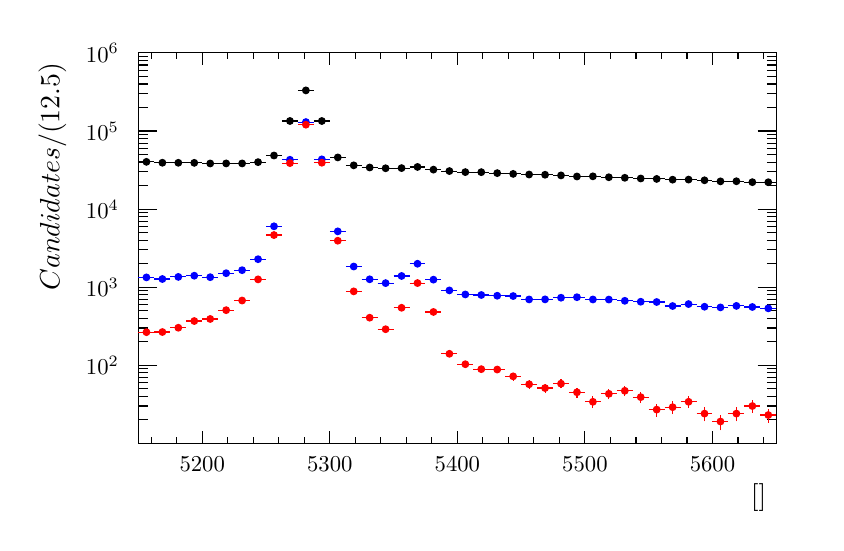
\begin{tikzpicture}
\pgfdeclareplotmark{cross} {
\pgfpathmoveto{\pgfpoint{-0.3\pgfplotmarksize}{\pgfplotmarksize}}
\pgfpathlineto{\pgfpoint{+0.3\pgfplotmarksize}{\pgfplotmarksize}}
\pgfpathlineto{\pgfpoint{+0.3\pgfplotmarksize}{0.3\pgfplotmarksize}}
\pgfpathlineto{\pgfpoint{+1\pgfplotmarksize}{0.3\pgfplotmarksize}}
\pgfpathlineto{\pgfpoint{+1\pgfplotmarksize}{-0.3\pgfplotmarksize}}
\pgfpathlineto{\pgfpoint{+0.3\pgfplotmarksize}{-0.3\pgfplotmarksize}}
\pgfpathlineto{\pgfpoint{+0.3\pgfplotmarksize}{-1.\pgfplotmarksize}}
\pgfpathlineto{\pgfpoint{-0.3\pgfplotmarksize}{-1.\pgfplotmarksize}}
\pgfpathlineto{\pgfpoint{-0.3\pgfplotmarksize}{-0.3\pgfplotmarksize}}
\pgfpathlineto{\pgfpoint{-1.\pgfplotmarksize}{-0.3\pgfplotmarksize}}
\pgfpathlineto{\pgfpoint{-1.\pgfplotmarksize}{0.3\pgfplotmarksize}}
\pgfpathlineto{\pgfpoint{-0.3\pgfplotmarksize}{0.3\pgfplotmarksize}}
\pgfpathclose
\pgfusepathqstroke
}
\pgfdeclareplotmark{cross*} {
\pgfpathmoveto{\pgfpoint{-0.3\pgfplotmarksize}{\pgfplotmarksize}}
\pgfpathlineto{\pgfpoint{+0.3\pgfplotmarksize}{\pgfplotmarksize}}
\pgfpathlineto{\pgfpoint{+0.3\pgfplotmarksize}{0.3\pgfplotmarksize}}
\pgfpathlineto{\pgfpoint{+1\pgfplotmarksize}{0.3\pgfplotmarksize}}
\pgfpathlineto{\pgfpoint{+1\pgfplotmarksize}{-0.3\pgfplotmarksize}}
\pgfpathlineto{\pgfpoint{+0.3\pgfplotmarksize}{-0.3\pgfplotmarksize}}
\pgfpathlineto{\pgfpoint{+0.3\pgfplotmarksize}{-1.\pgfplotmarksize}}
\pgfpathlineto{\pgfpoint{-0.3\pgfplotmarksize}{-1.\pgfplotmarksize}}
\pgfpathlineto{\pgfpoint{-0.3\pgfplotmarksize}{-0.3\pgfplotmarksize}}
\pgfpathlineto{\pgfpoint{-1.\pgfplotmarksize}{-0.3\pgfplotmarksize}}
\pgfpathlineto{\pgfpoint{-1.\pgfplotmarksize}{0.3\pgfplotmarksize}}
\pgfpathlineto{\pgfpoint{-0.3\pgfplotmarksize}{0.3\pgfplotmarksize}}
\pgfpathclose
\pgfusepathqfillstroke
}
\pgfdeclareplotmark{newstar} {
\pgfpathmoveto{\pgfqpoint{0pt}{\pgfplotmarksize}}
\pgfpathlineto{\pgfqpointpolar{44}{0.5\pgfplotmarksize}}
\pgfpathlineto{\pgfqpointpolar{18}{\pgfplotmarksize}}
\pgfpathlineto{\pgfqpointpolar{-20}{0.5\pgfplotmarksize}}
\pgfpathlineto{\pgfqpointpolar{-54}{\pgfplotmarksize}}
\pgfpathlineto{\pgfqpointpolar{-90}{0.5\pgfplotmarksize}}
\pgfpathlineto{\pgfqpointpolar{234}{\pgfplotmarksize}}
\pgfpathlineto{\pgfqpointpolar{198}{0.5\pgfplotmarksize}}
\pgfpathlineto{\pgfqpointpolar{162}{\pgfplotmarksize}}
\pgfpathlineto{\pgfqpointpolar{134}{0.5\pgfplotmarksize}}
\pgfpathclose
\pgfusepathqstroke
}
\pgfdeclareplotmark{newstar*} {
\pgfpathmoveto{\pgfqpoint{0pt}{\pgfplotmarksize}}
\pgfpathlineto{\pgfqpointpolar{44}{0.5\pgfplotmarksize}}
\pgfpathlineto{\pgfqpointpolar{18}{\pgfplotmarksize}}
\pgfpathlineto{\pgfqpointpolar{-20}{0.5\pgfplotmarksize}}
\pgfpathlineto{\pgfqpointpolar{-54}{\pgfplotmarksize}}
\pgfpathlineto{\pgfqpointpolar{-90}{0.5\pgfplotmarksize}}
\pgfpathlineto{\pgfqpointpolar{234}{\pgfplotmarksize}}
\pgfpathlineto{\pgfqpointpolar{198}{0.5\pgfplotmarksize}}
\pgfpathlineto{\pgfqpointpolar{162}{\pgfplotmarksize}}
\pgfpathlineto{\pgfqpointpolar{134}{0.5\pgfplotmarksize}}
\pgfpathclose
\pgfusepathqfillstroke
}
\definecolor{c}{rgb}{1,1,1};
\draw [color=c, fill=c] (0,0) rectangle (10,6.27517);
\draw [color=c, fill=c] (1.4,1.00403) rectangle (9.5,5.96141);
\definecolor{c}{rgb}{0,0,0};
\draw [c] (1.4,1.00403) -- (1.4,5.96141) -- (9.5,5.96141) -- (9.5,1.00403) -- (1.4,1.00403);
\draw [c,line width=0.4] (1.4,4.57797) -- (1.46769,4.57797);
\draw [c,line width=0.4] (1.53481,4.57797) -- (1.6025,4.57797);
\foreach \P in {(1.50125,4.57797)}{\draw[mark options={color=c,fill=c},mark size=1.201201pt,mark=*] plot coordinates {\P};}
\draw [c,line width=0.4] (1.6025,4.56676) -- (1.67019,4.56676);
\draw [c,line width=0.4] (1.73731,4.56676) -- (1.805,4.56676);
\foreach \P in {(1.70375,4.56676)}{\draw[mark options={color=c,fill=c},mark size=1.201201pt,mark=*] plot coordinates {\P};}
\draw [c,line width=0.4] (1.805,4.56614) -- (1.87269,4.56614);
\draw [c,line width=0.4] (1.93981,4.56614) -- (2.0075,4.56614);
\foreach \P in {(1.90625,4.56614)}{\draw[mark options={color=c,fill=c},mark size=1.201201pt,mark=*] plot coordinates {\P};}
\draw [c,line width=0.4] (2.0075,4.56542) -- (2.07519,4.56542);
\draw [c,line width=0.4] (2.14231,4.56542) -- (2.21,4.56542);
\foreach \P in {(2.10875,4.56542)}{\draw[mark options={color=c,fill=c},mark size=1.201201pt,mark=*] plot coordinates {\P};}
\draw [c,line width=0.4] (2.21,4.55762) -- (2.27769,4.55762);
\draw [c,line width=0.4] (2.34481,4.55762) -- (2.4125,4.55762);
\foreach \P in {(2.31125,4.55762)}{\draw[mark options={color=c,fill=c},mark size=1.201201pt,mark=*] plot coordinates {\P};}
\draw [c,line width=0.4] (2.4125,4.55827) -- (2.48019,4.55827);
\draw [c,line width=0.4] (2.54731,4.55827) -- (2.615,4.55827);
\foreach \P in {(2.51375,4.55827)}{\draw[mark options={color=c,fill=c},mark size=1.201201pt,mark=*] plot coordinates {\P};}
\draw [c,line width=0.4] (2.615,4.55815) -- (2.68269,4.55815);
\draw [c,line width=0.4] (2.74981,4.55815) -- (2.8175,4.55815);
\foreach \P in {(2.71625,4.55815)}{\draw[mark options={color=c,fill=c},mark size=1.201201pt,mark=*] plot coordinates {\P};}
\draw [c,line width=0.4] (2.8175,4.57444) -- (2.88519,4.57444);
\draw [c,line width=0.4] (2.95231,4.57444) -- (3.02,4.57444);
\foreach \P in {(2.91875,4.57444)}{\draw[mark options={color=c,fill=c},mark size=1.201201pt,mark=*] plot coordinates {\P};}
\draw [c,line width=0.4] (3.02,4.65853) -- (3.08769,4.65853);
\draw [c,line width=0.4] (3.15481,4.65853) -- (3.2225,4.65853);
\foreach \P in {(3.12125,4.65853)}{\draw[mark options={color=c,fill=c},mark size=1.201201pt,mark=*] plot coordinates {\P};}
\draw [c,line width=0.4] (3.2225,5.09721) -- (3.29019,5.09721);
\draw [c,line width=0.4] (3.35731,5.09721) -- (3.425,5.09721);
\foreach \P in {(3.32375,5.09721)}{\draw[mark options={color=c,fill=c},mark size=1.201201pt,mark=*] plot coordinates {\P};}
\draw [c,line width=0.4] (3.425,5.4856) -- (3.49269,5.4856);
\draw [c,line width=0.4] (3.55981,5.4856) -- (3.6275,5.4856);
\foreach \P in {(3.52625,5.4856)}{\draw[mark options={color=c,fill=c},mark size=1.201201pt,mark=*] plot coordinates {\P};}
\draw [c,line width=0.4] (3.6275,5.09678) -- (3.69519,5.09678);
\draw [c,line width=0.4] (3.76231,5.09678) -- (3.83,5.09678);
\foreach \P in {(3.72875,5.09678)}{\draw[mark options={color=c,fill=c},mark size=1.201201pt,mark=*] plot coordinates {\P};}
\draw [c,line width=0.4] (3.83,4.63432) -- (3.89769,4.63432);
\draw [c,line width=0.4] (3.96481,4.63432) -- (4.0325,4.63432);
\foreach \P in {(3.93125,4.63432)}{\draw[mark options={color=c,fill=c},mark size=1.201201pt,mark=*] plot coordinates {\P};}
\draw [c,line width=0.4] (4.0325,4.53369) -- (4.10019,4.53369);
\draw [c,line width=0.4] (4.16731,4.53369) -- (4.235,4.53369);
\foreach \P in {(4.13375,4.53369)}{\draw[mark options={color=c,fill=c},mark size=1.201201pt,mark=*] plot coordinates {\P};}
\draw [c,line width=0.4] (4.235,4.50656) -- (4.30269,4.50656);
\draw [c,line width=0.4] (4.36981,4.50656) -- (4.4375,4.50656);
\foreach \P in {(4.33625,4.50656)}{\draw[mark options={color=c,fill=c},mark size=1.201201pt,mark=*] plot coordinates {\P};}
\draw [c,line width=0.4] (4.4375,4.49664) -- (4.50519,4.49664);
\draw [c,line width=0.4] (4.57231,4.49664) -- (4.64,4.49664);
\foreach \P in {(4.53875,4.49664)}{\draw[mark options={color=c,fill=c},mark size=1.201201pt,mark=*] plot coordinates {\P};}
\draw [c,line width=0.4] (4.64,4.49881) -- (4.70769,4.49881);
\draw [c,line width=0.4] (4.77481,4.49881) -- (4.8425,4.49881);
\foreach \P in {(4.74125,4.49881)}{\draw[mark options={color=c,fill=c},mark size=1.201201pt,mark=*] plot coordinates {\P};}
\draw [c,line width=0.4] (4.8425,4.51337) -- (4.91019,4.51337);
\draw [c,line width=0.4] (4.97731,4.51337) -- (5.045,4.51337);
\foreach \P in {(4.94375,4.51337)}{\draw[mark options={color=c,fill=c},mark size=1.201201pt,mark=*] plot coordinates {\P};}
\draw [c,line width=0.4] (5.045,4.47929) -- (5.11269,4.47929);
\draw [c,line width=0.4] (5.17981,4.47929) -- (5.2475,4.47929);
\foreach \P in {(5.14625,4.47929)}{\draw[mark options={color=c,fill=c},mark size=1.201201pt,mark=*] plot coordinates {\P};}
\draw [c,line width=0.4] (5.2475,4.46118) -- (5.31519,4.46118);
\draw [c,line width=0.4] (5.38231,4.46118) -- (5.45,4.46118);
\foreach \P in {(5.34875,4.46118)}{\draw[mark options={color=c,fill=c},mark size=1.201201pt,mark=*] plot coordinates {\P};}
\draw [c,line width=0.4] (5.45,4.44797) -- (5.51769,4.44797);
\draw [c,line width=0.4] (5.58481,4.44797) -- (5.6525,4.44797);
\foreach \P in {(5.55125,4.44797)}{\draw[mark options={color=c,fill=c},mark size=1.201201pt,mark=*] plot coordinates {\P};}
\draw [c,line width=0.4] (5.6525,4.4472) -- (5.72019,4.4472);
\draw [c,line width=0.4] (5.78731,4.4472) -- (5.855,4.4472);
\foreach \P in {(5.75375,4.4472)}{\draw[mark options={color=c,fill=c},mark size=1.201201pt,mark=*] plot coordinates {\P};}
\draw [c,line width=0.4] (5.855,4.43495) -- (5.92269,4.43495);
\draw [c,line width=0.4] (5.98981,4.43495) -- (6.0575,4.43495);
\foreach \P in {(5.95625,4.43495)}{\draw[mark options={color=c,fill=c},mark size=1.201201pt,mark=*] plot coordinates {\P};}
\draw [c,line width=0.4] (6.0575,4.42534) -- (6.12519,4.42534);
\draw [c,line width=0.4] (6.19231,4.42534) -- (6.26,4.42534);
\foreach \P in {(6.15875,4.42534)}{\draw[mark options={color=c,fill=c},mark size=1.201201pt,mark=*] plot coordinates {\P};}
\draw [c,line width=0.4] (6.26,4.41737) -- (6.32769,4.41737);
\draw [c,line width=0.4] (6.39481,4.41737) -- (6.4625,4.41737);
\foreach \P in {(6.36125,4.41737)}{\draw[mark options={color=c,fill=c},mark size=1.201201pt,mark=*] plot coordinates {\P};}
\draw [c,line width=0.4] (6.4625,4.41444) -- (6.53019,4.41444);
\draw [c,line width=0.4] (6.59731,4.41444) -- (6.665,4.41444);
\foreach \P in {(6.56375,4.41444)}{\draw[mark options={color=c,fill=c},mark size=1.201201pt,mark=*] plot coordinates {\P};}
\draw [c,line width=0.4] (6.665,4.40594) -- (6.73269,4.40594);
\draw [c,line width=0.4] (6.79981,4.40594) -- (6.8675,4.40594);
\foreach \P in {(6.76625,4.40594)}{\draw[mark options={color=c,fill=c},mark size=1.201201pt,mark=*] plot coordinates {\P};}
\draw [c,line width=0.4] (6.8675,4.39235) -- (6.93519,4.39235);
\draw [c,line width=0.4] (7.00231,4.39235) -- (7.07,4.39235);
\foreach \P in {(6.96875,4.39235)}{\draw[mark options={color=c,fill=c},mark size=1.201201pt,mark=*] plot coordinates {\P};}
\draw [c,line width=0.4] (7.07,4.39413) -- (7.13769,4.39413);
\draw [c,line width=0.4] (7.20481,4.39413) -- (7.2725,4.39413);
\foreach \P in {(7.17125,4.39413)}{\draw[mark options={color=c,fill=c},mark size=1.201201pt,mark=*] plot coordinates {\P};}
\draw [c,line width=0.4] (7.2725,4.38246) -- (7.34019,4.38246);
\draw [c,line width=0.4] (7.40731,4.38246) -- (7.475,4.38246);
\foreach \P in {(7.37375,4.38246)}{\draw[mark options={color=c,fill=c},mark size=1.201201pt,mark=*] plot coordinates {\P};}
\draw [c,line width=0.4] (7.475,4.3756) -- (7.54269,4.3756);
\draw [c,line width=0.4] (7.60981,4.3756) -- (7.6775,4.3756);
\foreach \P in {(7.57625,4.3756)}{\draw[mark options={color=c,fill=c},mark size=1.201201pt,mark=*] plot coordinates {\P};}
\draw [c,line width=0.4] (7.6775,4.36671) -- (7.74519,4.36671);
\draw [c,line width=0.4] (7.81231,4.36671) -- (7.88,4.36671);
\foreach \P in {(7.77875,4.36671)}{\draw[mark options={color=c,fill=c},mark size=1.201201pt,mark=*] plot coordinates {\P};}
\draw [c,line width=0.4] (7.88,4.36129) -- (7.94769,4.36129);
\draw [c,line width=0.4] (8.01481,4.36129) -- (8.0825,4.36129);
\foreach \P in {(7.98125,4.36129)}{\draw[mark options={color=c,fill=c},mark size=1.201201pt,mark=*] plot coordinates {\P};}
\draw [c,line width=0.4] (8.0825,4.35166) -- (8.15019,4.35166);
\draw [c,line width=0.4] (8.21731,4.35166) -- (8.285,4.35166);
\foreach \P in {(8.18375,4.35166)}{\draw[mark options={color=c,fill=c},mark size=1.201201pt,mark=*] plot coordinates {\P};}
\draw [c,line width=0.4] (8.285,4.35293) -- (8.35269,4.35293);
\draw [c,line width=0.4] (8.41981,4.35293) -- (8.4875,4.35293);
\foreach \P in {(8.38625,4.35293)}{\draw[mark options={color=c,fill=c},mark size=1.201201pt,mark=*] plot coordinates {\P};}
\draw [c,line width=0.4] (8.4875,4.34392) -- (8.55519,4.34392);
\draw [c,line width=0.4] (8.62231,4.34392) -- (8.69,4.34392);
\foreach \P in {(8.58875,4.34392)}{\draw[mark options={color=c,fill=c},mark size=1.201201pt,mark=*] plot coordinates {\P};}
\draw [c,line width=0.4] (8.69,4.33029) -- (8.75769,4.33029);
\draw [c,line width=0.4] (8.82481,4.33029) -- (8.8925,4.33029);
\foreach \P in {(8.79125,4.33029)}{\draw[mark options={color=c,fill=c},mark size=1.201201pt,mark=*] plot coordinates {\P};}
\draw [c,line width=0.4] (8.8925,4.33171) -- (8.96019,4.33171);
\draw [c,line width=0.4] (9.02731,4.33171) -- (9.095,4.33171);
\foreach \P in {(8.99375,4.33171)}{\draw[mark options={color=c,fill=c},mark size=1.201201pt,mark=*] plot coordinates {\P};}
\draw [c,line width=0.4] (9.095,4.32015) -- (9.16269,4.32015);
\draw [c,line width=0.4] (9.22981,4.32015) -- (9.2975,4.32015);
\foreach \P in {(9.19625,4.32015)}{\draw[mark options={color=c,fill=c},mark size=1.201201pt,mark=*] plot coordinates {\P};}
\draw [c,line width=0.4] (9.2975,4.31923) -- (9.36519,4.31923);
\draw [c,line width=0.4] (9.43231,4.31923) -- (9.5,4.31923);
\foreach \P in {(9.39875,4.31923)}{\draw[mark options={color=c,fill=c},mark size=1.201201pt,mark=*] plot coordinates {\P};}
\draw [c,line width=0.4] (1.4,1.00403) -- (9.5,1.00403);
\draw [anchor= east] (9.5,0.317272) node[scale=1.00614, rotate=0]{\mJpsiKpi [\mevcc]};
\draw [c,line width=0.4] (2.21,1.15651) -- (2.21,1.00403);
\draw [c,line width=0.4] (2.534,1.08027) -- (2.534,1.00403);
\draw [c,line width=0.4] (2.858,1.08027) -- (2.858,1.00403);
\draw [c,line width=0.4] (3.182,1.08027) -- (3.182,1.00403);
\draw [c,line width=0.4] (3.506,1.08027) -- (3.506,1.00403);
\draw [c,line width=0.4] (3.83,1.15651) -- (3.83,1.00403);
\draw [c,line width=0.4] (4.154,1.08027) -- (4.154,1.00403);
\draw [c,line width=0.4] (4.478,1.08027) -- (4.478,1.00403);
\draw [c,line width=0.4] (4.802,1.08027) -- (4.802,1.00403);
\draw [c,line width=0.4] (5.126,1.08027) -- (5.126,1.00403);
\draw [c,line width=0.4] (5.45,1.15651) -- (5.45,1.00403);
\draw [c,line width=0.4] (5.774,1.08027) -- (5.774,1.00403);
\draw [c,line width=0.4] (6.098,1.08027) -- (6.098,1.00403);
\draw [c,line width=0.4] (6.422,1.08027) -- (6.422,1.00403);
\draw [c,line width=0.4] (6.746,1.08027) -- (6.746,1.00403);
\draw [c,line width=0.4] (7.07,1.15651) -- (7.07,1.00403);
\draw [c,line width=0.4] (7.394,1.08027) -- (7.394,1.00403);
\draw [c,line width=0.4] (7.718,1.08027) -- (7.718,1.00403);
\draw [c,line width=0.4] (8.042,1.08027) -- (8.042,1.00403);
\draw [c,line width=0.4] (8.366,1.08027) -- (8.366,1.00403);
\draw [c,line width=0.4] (8.69,1.15651) -- (8.69,1.00403);
\draw [c,line width=0.4] (2.21,1.15651) -- (2.21,1.00403);
\draw [c,line width=0.4] (1.886,1.08027) -- (1.886,1.00403);
\draw [c,line width=0.4] (1.562,1.08027) -- (1.562,1.00403);
\draw [c,line width=0.4] (8.69,1.15651) -- (8.69,1.00403);
\draw [c,line width=0.4] (9.014,1.08027) -- (9.014,1.00403);
\draw [c,line width=0.4] (9.338,1.08027) -- (9.338,1.00403);
\draw [anchor=base] (2.21,0.640067) node[scale=0.819821, rotate=0]{5200};
\draw [anchor=base] (3.83,0.640067) node[scale=0.819821, rotate=0]{5300};
\draw [anchor=base] (5.45,0.640067) node[scale=0.819821, rotate=0]{5400};
\draw [anchor=base] (7.07,0.640067) node[scale=0.819821, rotate=0]{5500};
\draw [anchor=base] (8.69,0.640067) node[scale=0.819821, rotate=0]{5600};
\draw [c,line width=0.4] (1.4,5.96141) -- (9.5,5.96141);
\draw [c,line width=0.4] (2.21,5.80892) -- (2.21,5.96141);
\draw [c,line width=0.4] (2.534,5.88517) -- (2.534,5.96141);
\draw [c,line width=0.4] (2.858,5.88517) -- (2.858,5.96141);
\draw [c,line width=0.4] (3.182,5.88517) -- (3.182,5.96141);
\draw [c,line width=0.4] (3.506,5.88517) -- (3.506,5.96141);
\draw [c,line width=0.4] (3.83,5.80892) -- (3.83,5.96141);
\draw [c,line width=0.4] (4.154,5.88517) -- (4.154,5.96141);
\draw [c,line width=0.4] (4.478,5.88517) -- (4.478,5.96141);
\draw [c,line width=0.4] (4.802,5.88517) -- (4.802,5.96141);
\draw [c,line width=0.4] (5.126,5.88517) -- (5.126,5.96141);
\draw [c,line width=0.4] (5.45,5.80892) -- (5.45,5.96141);
\draw [c,line width=0.4] (5.774,5.88517) -- (5.774,5.96141);
\draw [c,line width=0.4] (6.098,5.88517) -- (6.098,5.96141);
\draw [c,line width=0.4] (6.422,5.88517) -- (6.422,5.96141);
\draw [c,line width=0.4] (6.746,5.88517) -- (6.746,5.96141);
\draw [c,line width=0.4] (7.07,5.80892) -- (7.07,5.96141);
\draw [c,line width=0.4] (7.394,5.88517) -- (7.394,5.96141);
\draw [c,line width=0.4] (7.718,5.88517) -- (7.718,5.96141);
\draw [c,line width=0.4] (8.042,5.88517) -- (8.042,5.96141);
\draw [c,line width=0.4] (8.366,5.88517) -- (8.366,5.96141);
\draw [c,line width=0.4] (8.69,5.80892) -- (8.69,5.96141);
\draw [c,line width=0.4] (2.21,5.80892) -- (2.21,5.96141);
\draw [c,line width=0.4] (1.886,5.88517) -- (1.886,5.96141);
\draw [c,line width=0.4] (1.562,5.88517) -- (1.562,5.96141);
\draw [c,line width=0.4] (8.69,5.80892) -- (8.69,5.96141);
\draw [c,line width=0.4] (9.014,5.88517) -- (9.014,5.96141);
\draw [c,line width=0.4] (9.338,5.88517) -- (9.338,5.96141);
\draw [c,line width=0.4] (1.4,1.00403) -- (1.4,5.96141);
\draw [anchor= east] (0.3056,5.96141) node[scale=1.00614, rotate=90]{$\text{Candidates} / (12.5 \mevcc)$};
\draw [c,line width=0.4] (1.5185,1.30249) -- (1.4,1.30249);
\draw [c,line width=0.4] (1.5185,1.47708) -- (1.4,1.47708);
\draw [c,line width=0.4] (1.5185,1.60095) -- (1.4,1.60095);
\draw [c,line width=0.4] (1.5185,1.69704) -- (1.4,1.69704);
\draw [c,line width=0.4] (1.5185,1.77554) -- (1.4,1.77554);
\draw [c,line width=0.4] (1.5185,1.84192) -- (1.4,1.84192);
\draw [c,line width=0.4] (1.5185,1.89942) -- (1.4,1.89942);
\draw [c,line width=0.4] (1.5185,1.95014) -- (1.4,1.95014);
\draw [c,line width=0.4] (1.637,1.9955) -- (1.4,1.9955);
\draw [anchor= east] (1.252,1.9955) node[scale=0.819821, rotate=0]{$10^{2}$};
\draw [c,line width=0.4] (1.5185,2.29397) -- (1.4,2.29397);
\draw [c,line width=0.4] (1.5185,2.46856) -- (1.4,2.46856);
\draw [c,line width=0.4] (1.5185,2.59243) -- (1.4,2.59243);
\draw [c,line width=0.4] (1.5185,2.68852) -- (1.4,2.68852);
\draw [c,line width=0.4] (1.5185,2.76702) -- (1.4,2.76702);
\draw [c,line width=0.4] (1.5185,2.8334) -- (1.4,2.8334);
\draw [c,line width=0.4] (1.5185,2.8909) -- (1.4,2.8909);
\draw [c,line width=0.4] (1.5185,2.94161) -- (1.4,2.94161);
\draw [c,line width=0.4] (1.637,2.98698) -- (1.4,2.98698);
\draw [anchor= east] (1.252,2.98698) node[scale=0.819821, rotate=0]{$10^{3}$};
\draw [c,line width=0.4] (1.5185,3.28544) -- (1.4,3.28544);
\draw [c,line width=0.4] (1.5185,3.46003) -- (1.4,3.46003);
\draw [c,line width=0.4] (1.5185,3.58391) -- (1.4,3.58391);
\draw [c,line width=0.4] (1.5185,3.67999) -- (1.4,3.67999);
\draw [c,line width=0.4] (1.5185,3.7585) -- (1.4,3.7585);
\draw [c,line width=0.4] (1.5185,3.82487) -- (1.4,3.82487);
\draw [c,line width=0.4] (1.5185,3.88237) -- (1.4,3.88237);
\draw [c,line width=0.4] (1.5185,3.93309) -- (1.4,3.93309);
\draw [c,line width=0.4] (1.637,3.97846) -- (1.4,3.97846);
\draw [anchor= east] (1.252,3.97846) node[scale=0.819821, rotate=0]{$10^{4}$};
\draw [c,line width=0.4] (1.5185,4.27692) -- (1.4,4.27692);
\draw [c,line width=0.4] (1.5185,4.45151) -- (1.4,4.45151);
\draw [c,line width=0.4] (1.5185,4.57538) -- (1.4,4.57538);
\draw [c,line width=0.4] (1.5185,4.67147) -- (1.4,4.67147);
\draw [c,line width=0.4] (1.5185,4.74997) -- (1.4,4.74997);
\draw [c,line width=0.4] (1.5185,4.81635) -- (1.4,4.81635);
\draw [c,line width=0.4] (1.5185,4.87385) -- (1.4,4.87385);
\draw [c,line width=0.4] (1.5185,4.92457) -- (1.4,4.92457);
\draw [c,line width=0.4] (1.637,4.96993) -- (1.4,4.96993);
\draw [anchor= east] (1.252,4.96993) node[scale=0.819821, rotate=0]{$10^{5}$};
\draw [c,line width=0.4] (1.5185,5.2684) -- (1.4,5.2684);
\draw [c,line width=0.4] (1.5185,5.44299) -- (1.4,5.44299);
\draw [c,line width=0.4] (1.5185,5.56686) -- (1.4,5.56686);
\draw [c,line width=0.4] (1.5185,5.66295) -- (1.4,5.66295);
\draw [c,line width=0.4] (1.5185,5.74145) -- (1.4,5.74145);
\draw [c,line width=0.4] (1.5185,5.80783) -- (1.4,5.80783);
\draw [c,line width=0.4] (1.5185,5.86533) -- (1.4,5.86533);
\draw [c,line width=0.4] (1.5185,5.91604) -- (1.4,5.91604);
\draw [c,line width=0.4] (1.637,5.96141) -- (1.4,5.96141);
\draw [anchor= east] (1.252,5.96141) node[scale=0.819821, rotate=0]{$10^{6}$};
\draw [c,line width=0.4] (9.5,1.00403) -- (9.5,5.96141);
\draw [c,line width=0.4] (9.3815,1.30249) -- (9.5,1.30249);
\draw [c,line width=0.4] (9.3815,1.47708) -- (9.5,1.47708);
\draw [c,line width=0.4] (9.3815,1.60095) -- (9.5,1.60095);
\draw [c,line width=0.4] (9.3815,1.69704) -- (9.5,1.69704);
\draw [c,line width=0.4] (9.3815,1.77554) -- (9.5,1.77554);
\draw [c,line width=0.4] (9.3815,1.84192) -- (9.5,1.84192);
\draw [c,line width=0.4] (9.3815,1.89942) -- (9.5,1.89942);
\draw [c,line width=0.4] (9.3815,1.95014) -- (9.5,1.95014);
\draw [c,line width=0.4] (9.263,1.9955) -- (9.5,1.9955);
\draw [c,line width=0.4] (9.3815,2.29397) -- (9.5,2.29397);
\draw [c,line width=0.4] (9.3815,2.46856) -- (9.5,2.46856);
\draw [c,line width=0.4] (9.3815,2.59243) -- (9.5,2.59243);
\draw [c,line width=0.4] (9.3815,2.68852) -- (9.5,2.68852);
\draw [c,line width=0.4] (9.3815,2.76702) -- (9.5,2.76702);
\draw [c,line width=0.4] (9.3815,2.8334) -- (9.5,2.8334);
\draw [c,line width=0.4] (9.3815,2.8909) -- (9.5,2.8909);
\draw [c,line width=0.4] (9.3815,2.94161) -- (9.5,2.94161);
\draw [c,line width=0.4] (9.263,2.98698) -- (9.5,2.98698);
\draw [c,line width=0.4] (9.3815,3.28544) -- (9.5,3.28544);
\draw [c,line width=0.4] (9.3815,3.46003) -- (9.5,3.46003);
\draw [c,line width=0.4] (9.3815,3.58391) -- (9.5,3.58391);
\draw [c,line width=0.4] (9.3815,3.67999) -- (9.5,3.67999);
\draw [c,line width=0.4] (9.3815,3.7585) -- (9.5,3.7585);
\draw [c,line width=0.4] (9.3815,3.82487) -- (9.5,3.82487);
\draw [c,line width=0.4] (9.3815,3.88237) -- (9.5,3.88237);
\draw [c,line width=0.4] (9.3815,3.93309) -- (9.5,3.93309);
\draw [c,line width=0.4] (9.263,3.97846) -- (9.5,3.97846);
\draw [c,line width=0.4] (9.3815,4.27692) -- (9.5,4.27692);
\draw [c,line width=0.4] (9.3815,4.45151) -- (9.5,4.45151);
\draw [c,line width=0.4] (9.3815,4.57538) -- (9.5,4.57538);
\draw [c,line width=0.4] (9.3815,4.67147) -- (9.5,4.67147);
\draw [c,line width=0.4] (9.3815,4.74997) -- (9.5,4.74997);
\draw [c,line width=0.4] (9.3815,4.81635) -- (9.5,4.81635);
\draw [c,line width=0.4] (9.3815,4.87385) -- (9.5,4.87385);
\draw [c,line width=0.4] (9.3815,4.92457) -- (9.5,4.92457);
\draw [c,line width=0.4] (9.263,4.96993) -- (9.5,4.96993);
\draw [c,line width=0.4] (9.3815,5.2684) -- (9.5,5.2684);
\draw [c,line width=0.4] (9.3815,5.44299) -- (9.5,5.44299);
\draw [c,line width=0.4] (9.3815,5.56686) -- (9.5,5.56686);
\draw [c,line width=0.4] (9.3815,5.66295) -- (9.5,5.66295);
\draw [c,line width=0.4] (9.3815,5.74145) -- (9.5,5.74145);
\draw [c,line width=0.4] (9.3815,5.80783) -- (9.5,5.80783);
\draw [c,line width=0.4] (9.3815,5.86533) -- (9.5,5.86533);
\draw [c,line width=0.4] (9.3815,5.91604) -- (9.5,5.91604);
\draw [c,line width=0.4] (9.263,5.96141) -- (9.5,5.96141);
\definecolor{c}{rgb}{0,0,1};
\draw [c,line width=0.4] (1.4,3.11075) -- (1.46769,3.11075);
\draw [c,line width=0.4] (1.53481,3.11075) -- (1.6025,3.11075);
\foreach \P in {(1.50125,3.11075)}{\draw[mark options={color=c,fill=c},mark size=1.201201pt,mark=*] plot coordinates {\P};}
\draw [c,line width=0.4] (1.6025,3.09024) -- (1.67019,3.09024);
\draw [c,line width=0.4] (1.73731,3.09024) -- (1.805,3.09024);
\foreach \P in {(1.70375,3.09024)}{\draw[mark options={color=c,fill=c},mark size=1.201201pt,mark=*] plot coordinates {\P};}
\draw [c,line width=0.4] (1.805,3.11684) -- (1.87269,3.11684);
\draw [c,line width=0.4] (1.93981,3.11684) -- (2.0075,3.11684);
\foreach \P in {(1.90625,3.11684)}{\draw[mark options={color=c,fill=c},mark size=1.201201pt,mark=*] plot coordinates {\P};}
\draw [c,line width=0.4] (2.0075,3.13217) -- (2.07519,3.13217);
\draw [c,line width=0.4] (2.14231,3.13217) -- (2.21,3.13217);
\foreach \P in {(2.10875,3.13217)}{\draw[mark options={color=c,fill=c},mark size=1.201201pt,mark=*] plot coordinates {\P};}
\draw [c,line width=0.4] (2.21,3.11332) -- (2.27769,3.11332);
\draw [c,line width=0.4] (2.34481,3.11332) -- (2.4125,3.11332);
\foreach \P in {(2.31125,3.11332)}{\draw[mark options={color=c,fill=c},mark size=1.201201pt,mark=*] plot coordinates {\P};}
\draw [c,line width=0.4] (2.4125,3.16386) -- (2.48019,3.16386);
\draw [c,line width=0.4] (2.54731,3.16386) -- (2.615,3.16386);
\foreach \P in {(2.51375,3.16386)}{\draw[mark options={color=c,fill=c},mark size=1.201201pt,mark=*] plot coordinates {\P};}
\draw [c,line width=0.4] (2.615,3.20235) -- (2.68269,3.20235);
\draw [c,line width=0.4] (2.74981,3.20235) -- (2.8175,3.20235);
\foreach \P in {(2.71625,3.20235)}{\draw[mark options={color=c,fill=c},mark size=1.201201pt,mark=*] plot coordinates {\P};}
\draw [c,line width=0.4] (2.8175,3.34168) -- (2.88519,3.34168);
\draw [c,line width=0.4] (2.95231,3.34168) -- (3.02,3.34168);
\foreach \P in {(2.91875,3.34168)}{\draw[mark options={color=c,fill=c},mark size=1.201201pt,mark=*] plot coordinates {\P};}
\draw [c,line width=0.4] (3.02,3.7595) -- (3.08769,3.7595);
\draw [c,line width=0.4] (3.15481,3.7595) -- (3.2225,3.7595);
\foreach \P in {(3.12125,3.7595)}{\draw[mark options={color=c,fill=c},mark size=1.201201pt,mark=*] plot coordinates {\P};}
\draw [c,line width=0.4] (3.2225,4.6049) -- (3.29019,4.6049);
\draw [c,line width=0.4] (3.35731,4.6049) -- (3.425,4.6049);
\foreach \P in {(3.32375,4.6049)}{\draw[mark options={color=c,fill=c},mark size=1.201201pt,mark=*] plot coordinates {\P};}
\draw [c,line width=0.4] (3.425,5.08343) -- (3.49269,5.08343);
\draw [c,line width=0.4] (3.55981,5.08343) -- (3.6275,5.08343);
\foreach \P in {(3.52625,5.08343)}{\draw[mark options={color=c,fill=c},mark size=1.201201pt,mark=*] plot coordinates {\P};}
\draw [c,line width=0.4] (3.6275,4.60977) -- (3.69519,4.60977);
\draw [c,line width=0.4] (3.76231,4.60977) -- (3.83,4.60977);
\foreach \P in {(3.72875,4.60977)}{\draw[mark options={color=c,fill=c},mark size=1.201201pt,mark=*] plot coordinates {\P};}
\draw [c,line width=0.4] (3.83,3.69539) -- (3.89769,3.69539);
\draw [c,line width=0.4] (3.96481,3.69539) -- (4.0325,3.69539);
\foreach \P in {(3.93125,3.69539)}{\draw[mark options={color=c,fill=c},mark size=1.201201pt,mark=*] plot coordinates {\P};}
\draw [c,line width=0.4] (4.0325,3.24884) -- (4.10019,3.24884);
\draw [c,line width=0.4] (4.16731,3.24884) -- (4.235,3.24884);
\foreach \P in {(4.13375,3.24884)}{\draw[mark options={color=c,fill=c},mark size=1.201201pt,mark=*] plot coordinates {\P};}
\draw [c,line width=0.4] (4.235,3.08649) -- (4.30269,3.08649);
\draw [c,line width=0.4] (4.36981,3.08649) -- (4.4375,3.08649);
\foreach \P in {(4.33625,3.08649)}{\draw[mark options={color=c,fill=c},mark size=1.201201pt,mark=*] plot coordinates {\P};}
\draw [c,line width=0.4] (4.4375,3.03808) -- (4.50519,3.03808);
\draw [c,line width=0.4] (4.57231,3.03808) -- (4.64,3.03808);
\foreach \P in {(4.53875,3.03808)}{\draw[mark options={color=c,fill=c},mark size=1.201201pt,mark=*] plot coordinates {\P};}
\draw [c,line width=0.4] (4.64,3.12878) -- (4.70769,3.12878);
\draw [c,line width=0.4] (4.77481,3.12878) -- (4.8425,3.12878);
\foreach \P in {(4.74125,3.12878)}{\draw[mark options={color=c,fill=c},mark size=1.201201pt,mark=*] plot coordinates {\P};}
\draw [c,line width=0.4] (4.8425,3.28393) -- (4.91019,3.28393);
\draw [c,line width=0.4] (4.97731,3.28393) -- (5.045,3.28393);
\foreach \P in {(4.94375,3.28393)}{\draw[mark options={color=c,fill=c},mark size=1.201201pt,mark=*] plot coordinates {\P};}
\draw [c,line width=0.4] (5.045,3.08203) -- (5.11269,3.08203);
\draw [c,line width=0.4] (5.17981,3.08203) -- (5.2475,3.08203);
\foreach \P in {(5.14625,3.08203)}{\draw[mark options={color=c,fill=c},mark size=1.201201pt,mark=*] plot coordinates {\P};}
\draw [c,line width=0.4] (5.2475,2.94542) -- (5.31519,2.94542);
\draw [c,line width=0.4] (5.38231,2.94542) -- (5.45,2.94542);
\foreach \P in {(5.34875,2.94542)}{\draw[mark options={color=c,fill=c},mark size=1.201201pt,mark=*] plot coordinates {\P};}
\draw [c,line width=0.4] (5.45,2.89411) -- (5.51769,2.89411);
\draw [c,line width=0.4] (5.58481,2.89411) -- (5.6525,2.89411);
\foreach \P in {(5.55125,2.89411)}{\draw[mark options={color=c,fill=c},mark size=1.201201pt,mark=*] plot coordinates {\P};}
\draw [c,line width=0.4] (5.6525,2.88711) -- (5.72019,2.88711);
\draw [c,line width=0.4] (5.78731,2.88711) -- (5.855,2.88711);
\foreach \P in {(5.75375,2.88711)}{\draw[mark options={color=c,fill=c},mark size=1.201201pt,mark=*] plot coordinates {\P};}
\draw [c,line width=0.4] (5.855,2.87778) -- (5.92269,2.87778);
\draw [c,line width=0.4] (5.98981,2.87778) -- (6.0575,2.87778);
\foreach \P in {(5.95625,2.87778)}{\draw[mark options={color=c,fill=c},mark size=1.201201pt,mark=*] plot coordinates {\P};}
\draw [c,line width=0.4] (6.0575,2.87388) -- (6.12519,2.87388);
\draw [c,line width=0.4] (6.19231,2.87388) -- (6.26,2.87388);
\foreach \P in {(6.15875,2.87388)}{\draw[mark options={color=c,fill=c},mark size=1.201201pt,mark=*] plot coordinates {\P};}
\draw [c,line width=0.4] (6.26,2.83093) -- (6.32769,2.83093);
\draw [c,line width=0.4] (6.39481,2.83093) -- (6.4625,2.83093);
\foreach \P in {(6.36125,2.83093)}{\draw[mark options={color=c,fill=c},mark size=1.201201pt,mark=*] plot coordinates {\P};}
\draw [c,line width=0.4] (6.4625,2.83155) -- (6.53019,2.83155);
\draw [c,line width=0.4] (6.59731,2.83155) -- (6.665,2.83155);
\foreach \P in {(6.56375,2.83155)}{\draw[mark options={color=c,fill=c},mark size=1.201201pt,mark=*] plot coordinates {\P};}
\draw [c,line width=0.4] (6.665,2.85265) -- (6.73269,2.85265);
\draw [c,line width=0.4] (6.79981,2.85265) -- (6.8675,2.85265);
\foreach \P in {(6.76625,2.85265)}{\draw[mark options={color=c,fill=c},mark size=1.201201pt,mark=*] plot coordinates {\P};}
\draw [c,line width=0.4] (6.8675,2.85907) -- (6.93519,2.85907);
\draw [c,line width=0.4] (7.00231,2.85907) -- (7.07,2.85907);
\foreach \P in {(6.96875,2.85907)}{\draw[mark options={color=c,fill=c},mark size=1.201201pt,mark=*] plot coordinates {\P};}
\draw [c,line width=0.4] (7.07,2.83031) -- (7.13769,2.83031);
\draw [c,line width=0.4] (7.20481,2.83031) -- (7.2725,2.83031);
\foreach \P in {(7.17125,2.83031)}{\draw[mark options={color=c,fill=c},mark size=1.201201pt,mark=*] plot coordinates {\P};}
\draw [c,line width=0.4] (7.2725,2.82907) -- (7.34019,2.82907);
\draw [c,line width=0.4] (7.40731,2.82907) -- (7.475,2.82907);
\foreach \P in {(7.37375,2.82907)}{\draw[mark options={color=c,fill=c},mark size=1.201201pt,mark=*] plot coordinates {\P};}
\draw [c,line width=0.4] (7.475,2.81325) -- (7.54269,2.81325);
\draw [c,line width=0.4] (7.60981,2.81325) -- (7.6775,2.81325);
\foreach \P in {(7.57625,2.81325)}{\draw[mark options={color=c,fill=c},mark size=1.201201pt,mark=*] plot coordinates {\P};}
\draw [c,line width=0.4] (7.6775,2.80149) -- (7.74519,2.80149);
\draw [c,line width=0.4] (7.81231,2.80149) -- (7.88,2.80149);
\foreach \P in {(7.77875,2.80149)}{\draw[mark options={color=c,fill=c},mark size=1.201201pt,mark=*] plot coordinates {\P};}
\draw [c,line width=0.4] (7.88,2.79816) -- (7.94769,2.79816);
\draw [c,line width=0.4] (8.01481,2.79816) -- (8.0825,2.79816);
\foreach \P in {(7.98125,2.79816)}{\draw[mark options={color=c,fill=c},mark size=1.201201pt,mark=*] plot coordinates {\P};}
\draw [c,line width=0.4] (8.0825,2.7472) -- (8.15019,2.7472);
\draw [c,line width=0.4] (8.21731,2.7472) -- (8.285,2.7472);
\foreach \P in {(8.18375,2.7472)}{\draw[mark options={color=c,fill=c},mark size=1.201201pt,mark=*] plot coordinates {\P};}
\draw [c,line width=0.4] (8.285,2.77202) -- (8.35269,2.77202);
\draw [c,line width=0.4] (8.41981,2.77202) -- (8.4875,2.77202);
\foreach \P in {(8.38625,2.77202)}{\draw[mark options={color=c,fill=c},mark size=1.201201pt,mark=*] plot coordinates {\P};}
\draw [c,line width=0.4] (8.4875,2.73808) -- (8.55519,2.73808);
\draw [c,line width=0.4] (8.62231,2.73808) -- (8.69,2.73808);
\foreach \P in {(8.58875,2.73808)}{\draw[mark options={color=c,fill=c},mark size=1.201201pt,mark=*] plot coordinates {\P};}
\draw [c,line width=0.4] (8.69,2.72956) -- (8.75769,2.72956);
\draw [c,line width=0.4] (8.82481,2.72956) -- (8.8925,2.72956);
\foreach \P in {(8.79125,2.72956)}{\draw[mark options={color=c,fill=c},mark size=1.201201pt,mark=*] plot coordinates {\P};}
\draw [c,line width=0.4] (8.8925,2.7487) -- (8.96019,2.7487);
\draw [c,line width=0.4] (9.02731,2.7487) -- (9.095,2.7487);
\foreach \P in {(8.99375,2.7487)}{\draw[mark options={color=c,fill=c},mark size=1.201201pt,mark=*] plot coordinates {\P};}
\draw [c,line width=0.4] (9.095,2.735) -- (9.16269,2.735);
\draw [c,line width=0.4] (9.22981,2.735) -- (9.2975,2.735);
\foreach \P in {(9.19625,2.735)}{\draw[mark options={color=c,fill=c},mark size=1.201201pt,mark=*] plot coordinates {\P};}
\draw [c,line width=0.4] (9.2975,2.71765) -- (9.36519,2.71765);
\draw [c,line width=0.4] (9.43231,2.71765) -- (9.5,2.71765);
\foreach \P in {(9.39875,2.71765)}{\draw[mark options={color=c,fill=c},mark size=1.201201pt,mark=*] plot coordinates {\P};}
\definecolor{c}{rgb}{1,0,0};
\draw [c,line width=0.4] (1.4,2.41514) -- (1.46769,2.41514);
\draw [c,line width=0.4] (1.53481,2.41514) -- (1.6025,2.41514);
\foreach \P in {(1.50125,2.41514)}{\draw[mark options={color=c,fill=c},mark size=1.201201pt,mark=*] plot coordinates {\P};}
\draw [c,line width=0.4] (1.6025,2.41676) -- (1.67019,2.41676);
\draw [c,line width=0.4] (1.73731,2.41676) -- (1.805,2.41676);
\foreach \P in {(1.70375,2.41676)}{\draw[mark options={color=c,fill=c},mark size=1.201201pt,mark=*] plot coordinates {\P};}
\draw [c,line width=0.4] (1.805,2.47142) -- (1.87269,2.47142);
\draw [c,line width=0.4] (1.93981,2.47142) -- (2.0075,2.47142);
\foreach \P in {(1.90625,2.47142)}{\draw[mark options={color=c,fill=c},mark size=1.201201pt,mark=*] plot coordinates {\P};}
\draw [c,line width=0.4] (2.0075,2.55653) -- (2.07519,2.55653);
\draw [c,line width=0.4] (2.14231,2.55653) -- (2.21,2.55653);
\foreach \P in {(2.10875,2.55653)}{\draw[mark options={color=c,fill=c},mark size=1.201201pt,mark=*] plot coordinates {\P};}
\draw [c,line width=0.4] (2.21,2.58263) -- (2.27769,2.58263);
\draw [c,line width=0.4] (2.34481,2.58263) -- (2.4125,2.58263);
\foreach \P in {(2.31125,2.58263)}{\draw[mark options={color=c,fill=c},mark size=1.201201pt,mark=*] plot coordinates {\P};}
\draw [c,line width=0.4] (2.4125,2.6945) -- (2.48019,2.6945);
\draw [c,line width=0.4] (2.54731,2.6945) -- (2.615,2.6945);
\foreach \P in {(2.51375,2.6945)}{\draw[mark options={color=c,fill=c},mark size=1.201201pt,mark=*] plot coordinates {\P};}
\draw [c,line width=0.4] (2.615,2.8171) -- (2.68269,2.8171);
\draw [c,line width=0.4] (2.74981,2.8171) -- (2.8175,2.8171);
\foreach \P in {(2.71625,2.8171)}{\draw[mark options={color=c,fill=c},mark size=1.201201pt,mark=*] plot coordinates {\P};}
\draw [c,line width=0.4] (2.8175,3.08547) -- (2.88519,3.08547);
\draw [c,line width=0.4] (2.95231,3.08547) -- (3.02,3.08547);
\foreach \P in {(2.91875,3.08547)}{\draw[mark options={color=c,fill=c},mark size=1.201201pt,mark=*] plot coordinates {\P};}
\draw [c,line width=0.4] (3.02,3.64847) -- (3.08769,3.64847);
\draw [c,line width=0.4] (3.15481,3.64847) -- (3.2225,3.64847);
\foreach \P in {(3.12125,3.64847)}{\draw[mark options={color=c,fill=c},mark size=1.201201pt,mark=*] plot coordinates {\P};}
\draw [c,line width=0.4] (3.2225,4.56211) -- (3.29019,4.56211);
\draw [c,line width=0.4] (3.35731,4.56211) -- (3.425,4.56211);
\foreach \P in {(3.32375,4.56211)}{\draw[mark options={color=c,fill=c},mark size=1.201201pt,mark=*] plot coordinates {\P};}
\draw [c,line width=0.4] (3.425,5.05) -- (3.49269,5.05);
\draw [c,line width=0.4] (3.55981,5.05) -- (3.6275,5.05);
\foreach \P in {(3.52625,5.05)}{\draw[mark options={color=c,fill=c},mark size=1.201201pt,mark=*] plot coordinates {\P};}
\draw [c,line width=0.4] (3.6275,4.56695) -- (3.69519,4.56695);
\draw [c,line width=0.4] (3.76231,4.56695) -- (3.83,4.56695);
\foreach \P in {(3.72875,4.56695)}{\draw[mark options={color=c,fill=c},mark size=1.201201pt,mark=*] plot coordinates {\P};}
\draw [c,line width=0.4] (3.83,3.57642) -- (3.89769,3.57642);
\draw [c,line width=0.4] (3.96481,3.57642) -- (4.0325,3.57642);
\foreach \P in {(3.93125,3.57642)}{\draw[mark options={color=c,fill=c},mark size=1.201201pt,mark=*] plot coordinates {\P};}
\draw [c,line width=0.4] (4.0325,2.9334) -- (4.10019,2.9334);
\draw [c,line width=0.4] (4.16731,2.9334) -- (4.235,2.9334);
\foreach \P in {(4.13375,2.9334)}{\draw[mark options={color=c,fill=c},mark size=1.201201pt,mark=*] plot coordinates {\P};}
\draw [c,line width=0.4] (4.235,2.59884) -- (4.30269,2.59884);
\draw [c,line width=0.4] (4.36981,2.59884) -- (4.4375,2.59884);
\foreach \P in {(4.33625,2.59884)}{\draw[mark options={color=c,fill=c},mark size=1.201201pt,mark=*] plot coordinates {\P};}
\draw [c,line width=0.4] (4.4375,2.45247) -- (4.50519,2.45247);
\draw [c,line width=0.4] (4.57231,2.45247) -- (4.64,2.45247);
\foreach \P in {(4.53875,2.45247)}{\draw[mark options={color=c,fill=c},mark size=1.201201pt,mark=*] plot coordinates {\P};}
\draw [c,line width=0.4] (4.64,2.72483) -- (4.70769,2.72483);
\draw [c,line width=0.4] (4.77481,2.72483) -- (4.8425,2.72483);
\foreach \P in {(4.74125,2.72483)}{\draw[mark options={color=c,fill=c},mark size=1.201201pt,mark=*] plot coordinates {\P};}
\draw [c,line width=0.4] (4.8425,3.03884) -- (4.91019,3.03884);
\draw [c,line width=0.4] (4.97731,3.03884) -- (5.045,3.03884);
\foreach \P in {(4.94375,3.03884)}{\draw[mark options={color=c,fill=c},mark size=1.201201pt,mark=*] plot coordinates {\P};}
\draw [c,line width=0.4] (5.045,2.67183) -- (5.11269,2.67183);
\draw [c,line width=0.4] (5.17981,2.67183) -- (5.2475,2.67183);
\foreach \P in {(5.14625,2.67183)}{\draw[mark options={color=c,fill=c},mark size=1.201201pt,mark=*] plot coordinates {\P};}
\draw [c,line width=0.4] (5.34875,2.10236) -- (5.34875,2.10683);
\draw [c,line width=0.4] (5.34875,2.17394) -- (5.34875,2.17532);
\draw [c,line width=0.4] (5.2475,2.14039) -- (5.31519,2.14039);
\draw [c,line width=0.4] (5.38231,2.14039) -- (5.45,2.14039);
\foreach \P in {(5.34875,2.14039)}{\draw[mark options={color=c,fill=c},mark size=1.201201pt,mark=*] plot coordinates {\P};}
\draw [c,line width=0.4] (5.55125,1.96356) -- (5.55125,1.97467);
\draw [c,line width=0.4] (5.55125,2.04179) -- (5.55125,2.0487);
\draw [c,line width=0.4] (5.45,2.00823) -- (5.51769,2.00823);
\draw [c,line width=0.4] (5.58481,2.00823) -- (5.6525,2.00823);
\foreach \P in {(5.55125,2.00823)}{\draw[mark options={color=c,fill=c},mark size=1.201201pt,mark=*] plot coordinates {\P};}
\draw [c,line width=0.4] (5.75375,1.89708) -- (5.75375,1.91177);
\draw [c,line width=0.4] (5.75375,1.97888) -- (5.75375,1.98871);
\draw [c,line width=0.4] (5.6525,1.94532) -- (5.72019,1.94532);
\draw [c,line width=0.4] (5.78731,1.94532) -- (5.855,1.94532);
\foreach \P in {(5.75375,1.94532)}{\draw[mark options={color=c,fill=c},mark size=1.201201pt,mark=*] plot coordinates {\P};}
\draw [c,line width=0.4] (5.95625,1.89192) -- (5.95625,1.9069);
\draw [c,line width=0.4] (5.95625,1.97402) -- (5.95625,1.98408);
\draw [c,line width=0.4] (5.855,1.94046) -- (5.92269,1.94046);
\draw [c,line width=0.4] (5.98981,1.94046) -- (6.0575,1.94046);
\foreach \P in {(5.95625,1.94046)}{\draw[mark options={color=c,fill=c},mark size=1.201201pt,mark=*] plot coordinates {\P};}
\draw [c,line width=0.4] (6.15875,1.80006) -- (6.15875,1.82049);
\draw [c,line width=0.4] (6.15875,1.88761) -- (6.15875,1.90202);
\draw [c,line width=0.4] (6.0575,1.85405) -- (6.12519,1.85405);
\draw [c,line width=0.4] (6.19231,1.85405) -- (6.26,1.85405);
\foreach \P in {(6.15875,1.85405)}{\draw[mark options={color=c,fill=c},mark size=1.201201pt,mark=*] plot coordinates {\P};}
\draw [c,line width=0.4] (6.36125,1.69228) -- (6.36125,1.7199);
\draw [c,line width=0.4] (6.36125,1.78702) -- (6.36125,1.80702);
\draw [c,line width=0.4] (6.26,1.75346) -- (6.32769,1.75346);
\draw [c,line width=0.4] (6.39481,1.75346) -- (6.4625,1.75346);
\foreach \P in {(6.36125,1.75346)}{\draw[mark options={color=c,fill=c},mark size=1.201201pt,mark=*] plot coordinates {\P};}
\draw [c,line width=0.4] (6.56375,1.64061) -- (6.56375,1.67201);
\draw [c,line width=0.4] (6.56375,1.73912) -- (6.56375,1.762);
\draw [c,line width=0.4] (6.4625,1.70557) -- (6.53019,1.70557);
\draw [c,line width=0.4] (6.59731,1.70557) -- (6.665,1.70557);
\foreach \P in {(6.56375,1.70557)}{\draw[mark options={color=c,fill=c},mark size=1.201201pt,mark=*] plot coordinates {\P};}
\draw [c,line width=0.4] (6.76625,1.70034) -- (6.76625,1.72739);
\draw [c,line width=0.4] (6.76625,1.7945) -- (6.76625,1.81407);
\draw [c,line width=0.4] (6.665,1.76095) -- (6.73269,1.76095);
\draw [c,line width=0.4] (6.79981,1.76095) -- (6.8675,1.76095);
\foreach \P in {(6.76625,1.76095)}{\draw[mark options={color=c,fill=c},mark size=1.201201pt,mark=*] plot coordinates {\P};}
\draw [c,line width=0.4] (6.96875,1.58216) -- (6.96875,1.61811);
\draw [c,line width=0.4] (6.96875,1.68523) -- (6.96875,1.7115);
\draw [c,line width=0.4] (6.8675,1.65167) -- (6.93519,1.65167);
\draw [c,line width=0.4] (7.00231,1.65167) -- (7.07,1.65167);
\foreach \P in {(6.96875,1.65167)}{\draw[mark options={color=c,fill=c},mark size=1.201201pt,mark=*] plot coordinates {\P};}
\draw [c,line width=0.4] (7.17125,1.44997) -- (7.17125,1.49742);
\draw [c,line width=0.4] (7.17125,1.56453) -- (7.17125,1.59913);
\draw [c,line width=0.4] (7.07,1.53098) -- (7.13769,1.53098);
\draw [c,line width=0.4] (7.20481,1.53098) -- (7.2725,1.53098);
\foreach \P in {(7.17125,1.53098)}{\draw[mark options={color=c,fill=c},mark size=1.201201pt,mark=*] plot coordinates {\P};}
\draw [c,line width=0.4] (7.37375,1.56085) -- (7.37375,1.59854);
\draw [c,line width=0.4] (7.37375,1.66565) -- (7.37375,1.69321);
\draw [c,line width=0.4] (7.2725,1.6321) -- (7.34019,1.6321);
\draw [c,line width=0.4] (7.40731,1.6321) -- (7.475,1.6321);
\foreach \P in {(7.37375,1.6321)}{\draw[mark options={color=c,fill=c},mark size=1.201201pt,mark=*] plot coordinates {\P};}
\draw [c,line width=0.4] (7.57625,1.60251) -- (7.57625,1.63684);
\draw [c,line width=0.4] (7.57625,1.70395) -- (7.57625,1.72903);
\draw [c,line width=0.4] (7.475,1.6704) -- (7.54269,1.6704);
\draw [c,line width=0.4] (7.60981,1.6704) -- (7.6775,1.6704);
\foreach \P in {(7.57625,1.6704)}{\draw[mark options={color=c,fill=c},mark size=1.201201pt,mark=*] plot coordinates {\P};}
\draw [c,line width=0.4] (7.77875,1.51491) -- (7.77875,1.5565);
\draw [c,line width=0.4] (7.77875,1.62361) -- (7.77875,1.65401);
\draw [c,line width=0.4] (7.6775,1.59005) -- (7.74519,1.59005);
\draw [c,line width=0.4] (7.81231,1.59005) -- (7.88,1.59005);
\foreach \P in {(7.77875,1.59005)}{\draw[mark options={color=c,fill=c},mark size=1.201201pt,mark=*] plot coordinates {\P};}
\draw [c,line width=0.4] (7.98125,1.33967) -- (7.98125,1.39816);
\draw [c,line width=0.4] (7.98125,1.46527) -- (7.98125,1.5075);
\draw [c,line width=0.4] (7.88,1.43171) -- (7.94769,1.43171);
\draw [c,line width=0.4] (8.01481,1.43171) -- (8.0825,1.43171);
\foreach \P in {(7.98125,1.43171)}{\draw[mark options={color=c,fill=c},mark size=1.201201pt,mark=*] plot coordinates {\P};}
\draw [c,line width=0.4] (8.18375,1.37403) -- (8.18375,1.42893);
\draw [c,line width=0.4] (8.18375,1.49604) -- (8.18375,1.53583);
\draw [c,line width=0.4] (8.0825,1.46248) -- (8.15019,1.46248);
\draw [c,line width=0.4] (8.21731,1.46248) -- (8.285,1.46248);
\foreach \P in {(8.18375,1.46248)}{\draw[mark options={color=c,fill=c},mark size=1.201201pt,mark=*] plot coordinates {\P};}
\draw [c,line width=0.4] (8.38625,1.44997) -- (8.38625,1.49742);
\draw [c,line width=0.4] (8.38625,1.56453) -- (8.38625,1.59913);
\draw [c,line width=0.4] (8.285,1.53098) -- (8.35269,1.53098);
\draw [c,line width=0.4] (8.41981,1.53098) -- (8.4875,1.53098);
\foreach \P in {(8.38625,1.53098)}{\draw[mark options={color=c,fill=c},mark size=1.201201pt,mark=*] plot coordinates {\P};}
\draw [c,line width=0.4] (8.58875,1.28269) -- (8.58875,1.34744);
\draw [c,line width=0.4] (8.58875,1.41455) -- (8.58875,1.46098);
\draw [c,line width=0.4] (8.4875,1.381) -- (8.55519,1.381);
\draw [c,line width=0.4] (8.62231,1.381) -- (8.69,1.381);
\foreach \P in {(8.58875,1.381)}{\draw[mark options={color=c,fill=c},mark size=1.201201pt,mark=*] plot coordinates {\P};}
\draw [c,line width=0.4] (8.79125,1.16819) -- (8.79125,1.24685);
\draw [c,line width=0.4] (8.79125,1.31396) -- (8.79125,1.36934);
\draw [c,line width=0.4] (8.69,1.2804) -- (8.75769,1.2804);
\draw [c,line width=0.4] (8.82481,1.2804) -- (8.8925,1.2804);
\foreach \P in {(8.79125,1.2804)}{\draw[mark options={color=c,fill=c},mark size=1.201201pt,mark=*] plot coordinates {\P};}
\draw [c,line width=0.4] (8.99375,1.28269) -- (8.99375,1.34744);
\draw [c,line width=0.4] (8.99375,1.41455) -- (8.99375,1.46098);
\draw [c,line width=0.4] (8.8925,1.381) -- (8.96019,1.381);
\draw [c,line width=0.4] (9.02731,1.381) -- (9.095,1.381);
\foreach \P in {(8.99375,1.381)}{\draw[mark options={color=c,fill=c},mark size=1.201201pt,mark=*] plot coordinates {\P};}
\draw [c,line width=0.4] (9.19625,1.39028) -- (9.19625,1.44352);
\draw [c,line width=0.4] (9.19625,1.51064) -- (9.19625,1.54929);
\draw [c,line width=0.4] (9.095,1.47708) -- (9.16269,1.47708);
\draw [c,line width=0.4] (9.22981,1.47708) -- (9.2975,1.47708);
\foreach \P in {(9.19625,1.47708)}{\draw[mark options={color=c,fill=c},mark size=1.201201pt,mark=*] plot coordinates {\P};}
\draw [c,line width=0.4] (9.39875,1.26198) -- (9.39875,1.32911);
\draw [c,line width=0.4] (9.39875,1.39623) -- (9.39875,1.44422);
\draw [c,line width=0.4] (9.2975,1.36267) -- (9.36519,1.36267);
\draw [c,line width=0.4] (9.43231,1.36267) -- (9.5,1.36267);
\foreach \P in {(9.39875,1.36267)}{\draw[mark options={color=c,fill=c},mark size=1.201201pt,mark=*] plot coordinates {\P};}
\end{tikzpicture}
